% IEEE standard conference template; to be used with:
%   spconf.sty  - LaTeX style file, and
%   IEEEbib.bst - IEEE bibliography style file.
% --------------------------------------------------------------------------

\documentclass[letterpaper]{article}
\usepackage{spconf,amsmath,amssymb,graphicx,fancyvrb,xcolor,booktabs,url}

% Example definitions.
% --------------------
% nice symbols for real and complex numbers
\newcommand{\R}[0]{\mathbb{R}}
\newcommand{\C}[0]{\mathbb{C}}

% bold paragraph titlesgemi
\newcommand{\mypar}[1]{{\bf #1.}}

% Title.
% ------
\title{Optimizing Single Core Interval-Masked Top-$K$ Pearson Correlation}
%
% Single address.
% ---------------
\name{Oliver Bergqvist, Andres Navarro Pedregal, Luhao Liu \quad (Team 41)}
\address{Department of Computer Science\\ ETH Zurich, Switzerland}

% For example:
% ------------
%\address{School\\
%		 Department\\
%		 Address}
%
% Two addresses (uncomment and modify for two-address case).
% ----------------------------------------------------------
%\twoauthors
%  {A. Author-one, B. Author-two\sthanks{Thanks to XYZ agency for funding.}}
%		 {School A-B\\
%		 Department A-B\\
%		 Address A-B}
%  {C. Author-three, D. Author-four\sthanks{The fourth author performed the work
%		 while at ...}}
%		 {School C-D\\
%		 Department C-D\\
%		 Address C-D}
%

\begin{document}
%\ninept
%
\maketitle
%

% \begin{itemize} 
% 	\item The hard page limit is 7 pages in this style. This excludes references and excludes the short, mandatory part on individual contributions (see end). 
% 	\item No appendix. 
% 	\item Do not reduce font size or use other tricks to squeeze. 
% 	\item The pdf is formatted in the American letter format, so may look a bit strange when printed out (and there is no real reason to do this).
% \end{itemize}

\begin{abstract}
We optimize an Interval-Masked Streaming Top-$K$ Pearson Correlation algorithm for a single core. In order to guarantee an "apples-to-apples" comparison in terms of FLOP-counts, we start from a logical baseline, that already exploits correlation matrix symmetry and a mathematically equivalent, optimized variance formula. We then apply a structured sequence of optimizations: instruction-level parallelism, explicit AVX2/FMA vectorization, $4\times2$ register blocking, and a feature reordering that turns the interval structure into early loop termination and contiguous memory access. On a Kaby Lake core, the final implementation reaches $10.4$ flops/cycle ($33\%$ of AVX2+FMA peak performance), a $53\times$ speedup over the logical baseline when features span $80\%$ of each row and $26\times$ when features only span $30\%$ of each row.
\end{abstract}

\section{Introduction}\label{sec:intro}

% Do not start the introduction with the abstract or a slightly modified
% version. What follows is a possible structure of the introduction.
% This structure can be modified, but the content should be the same. The introduction should definitely end on the first page and leave some space for the second section on the first page.

% The first task is to motivate what you do.  You can
% start general and zoom in one the specific problem you consider.  In
% the process you should have explained to the reader: what you are doing,
% why you are doing, why it is important (order is usually reversed).

% For example, if my result is the fastest DFT implementation ever, one
% could roughly go as follows. First explain why the DFT is important
% (used everywhere with a few examples) and why performance matters (large datasets,
% realtime). Then explain that fast implementations are very hard and
% expensive to get (memory hierarchy, vector, parallel). 

% List some related work on fast implementations for your project if available (in particular those that you compare against) and very briefly explain what they did.

\mypar{Motivation}
The computation of pairwise Pearson correlation coefficients \cite{pearson1895regression} across high-dimensional feature sets is a common operation in data analytics, used for example in gene co-expression modeling \cite{langfelder2008wgcna}.
As more data arrives as time-oriented streams, static matrix computations are increasingly replaced by dynamically windowed correlation tracking \cite{papadimitriou2006local}.
The Interval-Masked Streaming Top-$K$ Pearson Correlation algorithm addresses these demands by introducing dynamic filters on the valid ranges and streaming only the top-$K$ highest values, thereby avoiding the full materialization of the intermediate correlation matrix.

Optimizing this algorithm is harder than it first appears.
Tuned libraries such as BLAS reach peak performance only on dense data with uniform access patterns.
Interval masking, however, gives each feature pair its own start and end indices.
These non-uniform bounds break standard cache-blocking and add control-flow branching that hampers SIMD vectorization, so reaching high throughput requires a custom implementation.
Prior work addresses related but different problems. Schubert and Gertz \cite{schubert2018numerically} optimize the numerically stable computation of (co-)variance, which we adopt for our preprocessing, but they consider neither the partially overlapping intervals nor the top-$K$ selection. TOP-COP \cite{xiong2006topcop} mines the top-$K$ strongly correlated pairs, but its focus is on pruning the search algorithmically rather than on the single-core, vectorized execution we study here.

% Now you state what you do in this paper. In our example it could be:
% presenting a DFT implementation for sizes divisible by 4 that is optimized for locality and uses AVX SIMD operations. It is faster for some sizes $> 128$ than prior code. Be brief so you have space for the core part of the paper.

\mypar{Contribution}
In this report, we detail a series of software optimizations applied to the Interval-Masked Streaming Top-$K$ Pearson Correlation algorithm executing on a single CPU core.
Using explicit vectorization, instruction-level parallelism (ILP), and cache-friendly data reordering, our optimized C++ implementation substantially outperforms the straightforward baseline.
For a problem size of 2048 features across 512 dimensions, we achieve: (1) a $53\times$ speedup when $80\%$ of the values fall within the valid interval, and (2) a $26\times$ speedup when only $30\%$ of the values are valid, both measured against the logical baseline.


\section{Background on the Algorithm}\label{sec:background}

% Give a short summary on the algorithm or application that you then later optimize. Show some of the key parts or equations. {\bf Then define the cost measure and show the cost analysis that you later use to create performance plots.}

\mypar{Algorithm}
The Interval-Masked Streaming Top-$K$ Pearson Correlation algorithm is designed to identify the $K$ most strongly correlated features for every feature within a high-dimensional dataset, constrained by feature-specific valid intervals.
Given the input data matrix $X$ of size $F \times S$ (features $\times$ dimensions/samples per feature), along with two arrays, $\text{start}$ and $\text{end}$, of length $F$ that define the valid interval $[\text{start}[f], \text{end}[f])$ for each feature, the algorithm executes in three distinct phases:

\textbf{Phase 1: Preprocessing.}
For each feature $f \in F$, the algorithm isolates the valid data window to compute the local mean ($\mu_f$) and sample standard deviation ($\sigma_f$).
Let $S_f = \text{start}[f]$, $E_f = \text{end}[f]$, and the interval length $N_f = E_f - S_f$.
The statistics can be shown as:

$$ \mu_f = \frac{1}{N_f} \sum_{i=S_f}^{E_f - 1} X_{f,i} \quad
\sigma_f = \sqrt{\frac{1}{N_f - 1} \sum_{i=S_f}^{E_f - 1} (X_{f,i} - \mu_f)^2} $$

In the actual algorithm, the $\sigma_f$ is calculated using the mathematical relation between mean and variance: 

% $$  \sigma_f = \sqrt{\frac{1}{N_f - 1} (\sum_{i=S_f}^{E_f - 1} X_{f,i}^2 - 2.0 \times \mu_f  \sum_{i=S_f}^{E_f - 1} X_{f,i} + N_f \mu_f^2) } $$
$$ \sigma^2 = \frac{1}{n-1} \sum (x - \mu)^2 = \frac{1}{n-1}(\sum x^2 - 2 \mu \sum x + \mu^2) $$

Further, the $z$-normalized values ($z_{f, i} = \frac{(X_{f, i} - \mu_{f})}{\sigma_{f}}$) are also pre-computed here to avoid repeated calculations in Phase 2.

\textbf{Phase 2: Overlap Correlation Calculation.}
For every unique pair of features $f_0$ and $f_1$, the algorithm determines the strict overlap of their valid intervals.
The bounds of this overlapping region are defined by $L = \max(S_{f_0}, S_{f_1})$ and $R = \min(E_{f_0}, E_{f_1})$. 

Assuming a meaningful overlap exists (i.e., $R - L > 1$), let the overlap length be $O = R - L$.
The interval-masked Pearson correlation coefficient ($\rho_{f_0, f_1}$) is then calculated by taking the dot product of the $z$-normalized values within this specific overlapping window:

$$ \rho_{f_0, f_1} = \frac{1}{O - 1} \sum_{i=L}^{R-1} z_{f_0, i} z_{f_1, i} $$

Since $\rho_{f0, f1} = \rho_{f1, f0}$, only the upper half triangular ($f_1 > f_0$) is actually computed in the algorithm. Note that self correlations are excluded in our setup.

\textbf{Phase 3: Streaming Top-$K$ Selection.}
Rather than storing the full $O(F^2)$ correlation matrix, the algorithm streams the calculated coefficients into a bounded selection data structure (such as a min-heap of size $K$).
For each feature $f_0$, it maintains only the $K$ indices of $f_1$ that yield the highest values of $\rho_{f_0, f_1}$.
The final output is an $F \times K$ index matrix representing the top-$K$ correlated peers for every feature.

\mypar{Cost Analysis}
We solely focus on the floating point arithmetic for cost analysis.
In Phase 1, for each feature $f$ with valid values $N_f$, $N_f$ FLOPs are needed to accumulate the values, $2N_f$ FLOPs to accumulate the square of values and $2N_f$ FLOPs for normalization. An additional $10$ FLOPs are also necessary for the calculation of $\mu_f$ and $\sigma_f$.
In Phase 2, for each valid pair $(f_0, f_1)$ where $f_1 > f_0$ with $O_{f0, f1}$ overlapping values, $2O_{f0, f1}$ FLOPs are needed to accumulate the multiplications and $1$ additional FLOP to perform the division.
In Phase 3, no FLOPs are counted as we do not perform any arithmetic computation directly.

In total, we have a total cost in FLOPs of

$$ \sum_{f \in F} (5N_f + 10) + \sum_{(f0, f1) \in (F, F), f_1 > f_0} (2O_{f_0, f_1} + 1) $$

In terms of data transfer, we only count compulsory misses, which consist of the input matrix, the normalized matrix, the heap insertions, and the final top-$K$ results. 

$$ (4 \times \sum_{f \in F} 2N_f) + (8 \times F \times K) + (4 \times F \times K) \text{ Bytes} $$

\section{Optimization Performed}\label{sec:yourmethod}

% Now comes the ``beef'' of the paper, where you explain what you
% did. Again, organize it in paragraphs with titles. As in every section
% you start with a very brief overview of the section.

% For this course, explain all the optimizations you performed. This mean, you first very briefly
% explain the baseline implementation, then go through locality and other optimizations, and finally SSE (every project will be slightly different of course). Show or mention relevant analysis or assumptions. A few examples: 1) Profiling may lead you to optimize one part first; 2) bandwidth plus data transfer analysis may show that it is memory bound; 3) it may be too hard to implement the algorithm in full generality: make assumptions and state them (e.g., we assume $n$ is divisible by 4; or, we consider only one type of input image); 4) explain how certain data accesses have poor locality. Generally, any type of analysis adds value to your work.

% As important as the final results is to show that you took a structured, organized approach to the optimization and that you explain why you did what you did.

% Mention and cite any external resources including library or other code.

% Good visuals or even brief code snippets to illustrate what you did are good. Pasting large amounts of code or screen shots to fill the space is not good.

\mypar{Logical Baseline}
The logical baseline is implemented exactly as described in Section \ref{sec:background}.
This baseline already incorporates several algorithmic reductions: variance formula rewriting, $z$-score normalization pre-computation, and the exploitation of the correlation matrix's symmetry.
We also implemented a purely naive baseline omitting these techniques, but they change the FLOP count and the underlying cost model.
Therefore, all subsequent analysis, profiling, and experiments refer to this logical baseline unless otherwise specified.

To identify the primary computational bottleneck, we conducted a runtime profiling using a problem size of $F = 128$ features and $S = 8192$ dimensions.
The profiling revealed that Phases 1, 2, and 3 account for 3.4\%, 96.6\%, and 0.1\% of the total CPU cycles, respectively.
This indicates that the Phase 2 inner loop—specifically the calculation of the dot product over the overlapping interval—dominates the execution time in the logical baseline.
Consequently, our primary optimizations are targeted at this specific loop:

{\fontsize{8}{10}\selectfont
\begin{Verbatim}
for (uint32_t t = L; t < R; ++t) {
    acc += Z[i*S + t] * Z[j*S + t];
}
corr = acc / (R - L - 1);
\end{Verbatim}
}

However, by Amdahl's Law, as pipelining-aware optimization and vectorization cut Phase 2's runtime, the formerly negligible Phases 1 and 3 account for a growing fraction of the total runtime.
To prevent these phases from emerging as secondary bottlenecks, the memory and vectorization optimizations discussed in the following sections are systematically applied to all phases wherever viable.

\mypar{ILP Optimization}
% (NOTE: This refers to 4_manual_ilp)
In the baseline implementation, the inner loop's accumulator depends directly on the computation from the previous iteration.
This loop-carried data dependency creates a strict read-after-write (RAW) hazard.
Because this hazard cannot be bypassed via hardware register renaming, it prevents the full utilization of the CPU pipeline and severely limits instruction-level parallelism (ILP).
To resolve this bottleneck, we split the reduction across several independent accumulators, which removes the single dependency chain and lets the out-of-order core overlap successive multiply-adds.
The loop is unrolled only as the mechanism that exposes these independent accumulators; the unrolling itself is not the source of the speedup.
The number of accumulators that is useful is dictated by the microarchitecture's instruction throughput and latency.
On the target Kaby Lake core (Skylake refresh microarchitecture), a Fused Multiply-Add (FMA) instruction has a latency of 4 cycles and can be issued twice per cycle, so 8 independent accumulators are needed to fully hide the execution latency.
In this scalar stage we use 4 accumulators, and reach the full 8 only later with the register-blocked vector kernel for simplicity.

{\fontsize{8}{10}\selectfont
\begin{Verbatim}
for (uint32_t t = L; t + 3 < R; t += 4) {
    acc0 += Z[i*S + t + 0] * Z[j*S + t + 0];
    acc1 += Z[i*S + t + 1] * Z[j*S + t + 1];
    acc2 += Z[i*S + t + 2] * Z[j*S + t + 2];
    acc3 += Z[i*S + t + 3] * Z[j*S + t + 3];
}
corr = (acc0 + acc1 + acc2 + acc3) / (R - L - 1);
\end{Verbatim}
}

Similar optimizations were also applied to Phase 1.
This configuration represents the highest-performing scalar version before the introduction of explicit vectorization.

\mypar{Vectorization}
% (NOTE: This refers to 5_manual_vectorization)
Next, we applied explicit vectorization to fully exploit the Single Instruction, Multiple Data (SIMD) capabilities of the CPU.
Because our normalized data is stored as 32-bit floating-point values, utilizing 256-bit Advanced Vector Extensions (AVX) instructions allows us to execute 8-way parallel computations.

{\fontsize{8}{10}\selectfont
\begin{Verbatim}
for (uint32_t t = L; t + 7 < R; t += 8) {
    __m256 v_i = _mm256_loadu_ps(&Z[i*S + t]);
    __m256 v_j = _mm256_loadu_ps(&Z[j*S + t]);
    v_acc = _mm256_fmadd_ps(v_i, v_j, v_acc);
}
float acc = hsum256(v_acc); // sum of all values
corr = acc / (R - L - 1);
\end{Verbatim}
}

While vectorization improves throughput, consolidating the inner loop into a single vector accumulator reintroduces a loop-carried data dependency.
ILP therefore drops, leaving the execution pipeline partially starved.
To resolve this pipeline underutilization and achieve peak performance, we reintroduced the multiple-accumulator strategy through blocking, which is detailed in the subsequent section.


\mypar{Blocking}
% (NOTE: This refers to 7_multi_accumulator)
For simplicity in our vectorized implementation, we assume that all interval boundaries, as well as the total dimension size $S$, are strictly divisible by 8.
For a fully generalized implementation, this constraint can be easily relaxed by aligning the start and end indices to the nearest multiple of 8, provided that the out-of-bounds normalized values are padded with zeros to ensure they do not affect the final accumulation.
Because this corner case has a negligible impact on our primary optimization goals, we opted to ignore it in our implementation.

Combining loop blocking (tiling) with vectorization yields two major architectural benefits: improved cache locality and restored ILP.
In Phase 2, the naive double outer loop iterates over feature pairs in a linear order: (0, 1), (0, 2), ..., (0, $F-1$), (1, 2), (1, 3), ....
When $F$ and $S$ become sufficiently large, the cache can no longer house the entire $Z$ matrix.
Under these conditions, only the values of the outer-loop feature are retained in the cache, while iterating through the inner loop triggers continuous cache evictions across the entire matrix.
To mitigate this, we restructured the computation into $4 \times 2$ blocks.
The access pattern is thus transformed into block-wise iterations:
([0, 1, 2, 3], [4, 5]), ([0, 1, 2, 3], [6, 7]), ..., ([0, 1, 2, 3], [$F-2$, $F-1$]), ([4, 5, 6, 7], [8, 9]), ...
(Note that the diagonal components, such as the correlations within the block $[0, 1, 2, 3]$ against itself, are computed via a specialized routine prior to entering the inner loop).
By evaluating a $4 \times 2$ block of the correlation matrix at once, the data loaded for the 4 outer features is reused across the 2 inner features, reducing memory traffic and the cache miss rate by a factor of four compared to the unblocked version.
Processing 8 independent feature pairs per iteration also uses 8 separate vector accumulators, enough to keep both FMA units busy and restore ILP.

The blocked kernel is long and intrinsic-heavy, so we omit the snippet here; the full source is in Section \ref{sec:code}.
Similar blocking and vectorization were also deployed in Phase 1.


\mypar{Sorting}
% (NOTE: This refers to 8_sorting)
An unclustered distribution of valid intervals degrades cache locality and incurs redundant memory accesses.
Pre-sorting the features by their starting indices lets us terminate the inner loop early: once a candidate feature's starting index exceeds the target feature's ending index, all subsequent features are disjoint and we can exit.
As shown in Figure \ref{fig:sorting_mechanism}, clustering by overlap also produces contiguous strips of accessed memory that fit better in the caches.
Iterating over these sorted blocks yields a predictable stride pattern, which improves the hardware prefetcher's hit rate.

\begin{figure}[htbp]
    \centering
    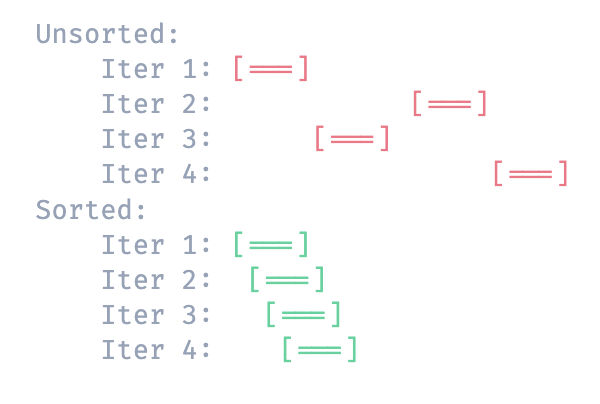
\includegraphics[trim=0mm 7mm 0mm 3mm, clip, width=0.55\linewidth]{figures/sorting_mechanism.png}
    \caption{Different access patterns before and after sorting.}
    \label{fig:sorting_mechanism}
\end{figure}

This data reordering mechanism is implemented alongside all previously discussed architectural optimizations.
During Phase 1, an initial sorting routine generates an index permutation array (Step 1), and the subsequent normalization routine physically reorders the rows of the $Z$ matrix in memory according to this permutation (Step 2).
In Phase 2, the min-heap insertion logic is updated to dereference the permutation array, ensuring the original feature indices are correctly preserved during the streaming Top-$K$ selection (Step 3).
Finally, in Phase 3, the output rows are scattered back into their original locations via the permutation array, ensuring the final output matrix remains consistent with the input data layout (Step 4).

{\fontsize{8}{10}\selectfont
\begin{Verbatim}
// Phase 1
// Step 1: sort by start
for (i) perm[i] = i;
std::sort(perm, perm+F, [&](a,b){start[a]<start[b]});
for (si) { // cache sorted bounds
  sorted_starts[si] = starts[perm[si]];
  sorted_ends[si]   = ends[perm[si]];
}
// Step 2: normalize, read original row
// perm[si], write sorted row si
Z[si*S + t] = (X[perm[si]*S+t] - mean) * inv_std;
// Phase 2
// Step 3: sorted-space dot-prod: orig. idx → heap
heap_insert(&heaps[i*K], v, perm[j]);
// Phase 3
// Step 4: scatter through perm
heap_to_topK(&heaps[si*K], &topK[perm[si]*K]);
\end{Verbatim}
}

The benefit of sorting depends on the density of the overlapping intervals.
With sparse intervals, the early-exit condition triggers often and prunes a large share of the evaluated pairs.
Conversely, when the intervals are dense and mostly overlap, the computational reduction is small, and the gains come instead from better cache locality and prefetch.


\section{Experimental Results}\label{sec:exp}
We evaluate each optimization by sweeping the number of features $F$ and the sample count $S$ separately. All experiments are run in both settings provided, dense (\texttt{LONG}) and sparse (\texttt{SHORT}), because the two stress the algorithm very differently. We answer the following questions: how much each step contributes to the latency, why $F$ and $S$ sweeps behave differently, how performance scales when scaling $F$ and $S$, and what limits the best code.

\mypar{Experimental setup}
All experiments are run on a single Kaby Lake core (Intel i7-7700HQ, Skylake-refresh microarchitecture) at a fixed $2.80$\,GHz, with $32$\,KB L1-D, $256$\,KB L2, and a $6$\,MB shared L3. To make the cycle counts reproducible we disable Turbo Boost, pin the frequency governor to \texttt{performance}, disable the core sibling so that nothing shares the physical core, and pin the benchmark to the core with \texttt{taskset}. The code is compiled with g++ $12.2.0$. The compilation flags vary in each step and are themselves part of the experiment. The logical baseline is left unoptimized (\texttt{-O0}). The two manual-ILP variants share identical source compiled with \texttt{-O3 -march=native -ffast-math} and differ only in whether the auto-vectorizer is turned off or not by \texttt{-fno-tree-vectorize}. The explicit-SIMD and sorting variants additionally enable \texttt{-mavx -mfma}. The single-precision AVX2+FMA peak on this core is $32$ flops/cycle ($2$ FMA units $\times\,8$ fp32 lanes $\times\,2$ flops).

We use PAPI \cite{papi} to count the cycles, instructions, cache misses, and flop counts to be able to understand the bottlenecks. We measure under cold-cache conditions: before each measured batch we \texttt{clflush} the input matrix, the interval bounds, and the output buffer. Each batch is sized to span at least $10^{8}$ cycles and one warm-up batch is discarded, so that timer and PAPI overhead are negligible. We report the median over the batches.

The inputs are generated synthetically by a provided generator. The $F$-sweep ranges over $F\in\{8,\dots,2048\}$ at a fixed $S=512$, and the $S$-sweep ranges over $S\in\{32,\dots,16384\}$ at a fixed $F=512$. The upper ends of both ranges are set by how long the experiments take rather than by the algorithm, because the slowest variant we measure is the unoptimized logical baseline and the total work grows quickly: the number of feature pairs grows as $F^2$ and the work per pair grows with $S$. In our runs the full $F$-sweep over all variants already took about six hours, and on the $S$-sweep a single baseline point cost about four hours at $S=8192$ and roughly doubled with each doubling of $S$, so that the complete $S$-sweep did not finish within $26$ hours and had to be stopped. We therefore cap the sweeps at $F=2048$ and $S=16384$, which is the largest range that still completes overnight while comfortably covering the transition from data fitting in cache to spilling to main memory. Each feature is given a fixed-length valid subinterval placed at a random offset (aligned to a multiple of $16$), and we report the top-$K$ neighbours with $K=16$. The interval length can be of two types, $80\%$ (\texttt{LONG}) or $30\%$ (\texttt{SHORT}) of the row. Sample values are i.i.d.\ Gaussian. As the algorithm does not depend on the values of the data, the performance is the same, regardless of how the data is generated. We tested that with the \texttt{BLOCK\_CORR} and \texttt{GAUSSIAN}, so we report only the Gaussian results. Throughout, the performance on the $y$-axis is the analytical useful-flop count of Section~\ref{sec:background} divided by the measured cycles. We want to be explicit about this choice, since we also record the hardware floating-point counter \texttt{PAPI\_SP\_OPS} and deliberately keep it off the axis. Because the SIMD kernels pad the invalid lanes with zeros, \texttt{PAPI\_SP\_OPS} also counts the arithmetic spent on that padding, which at $F=2048$ inflates the hardware count by up to $4.8\times$ on \texttt{SHORT} (the padding factor in Table~\ref{tab:papi}). Putting that hardware count on the axis would make the dense algorithm look fast on sparse data and make sorting, whose whole purpose is to remove the padding, appear as a slowdown. It would also break the rule of not comparing variants whose operation counts differ substantially. We therefore use the analytical count as the measure of useful work, and use \texttt{PAPI\_SP\_OPS} separately as a direct measurement of the padding overhead. Because the logical baseline already changes the operation count relative to a purely naive version, it is excluded from the plots and all speedups are against the logical baseline.

\begin{figure*}[h!]
  \centering
  
  % --- FIGURE 1 (Performance) ---
  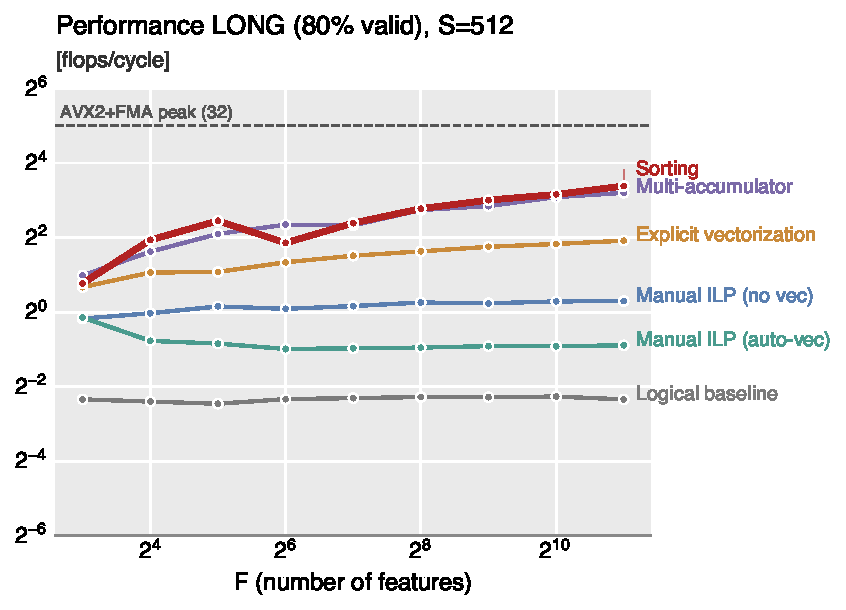
\includegraphics[width=0.48\linewidth]{figures/generated/perf_LONG.pdf}
  \hfill
  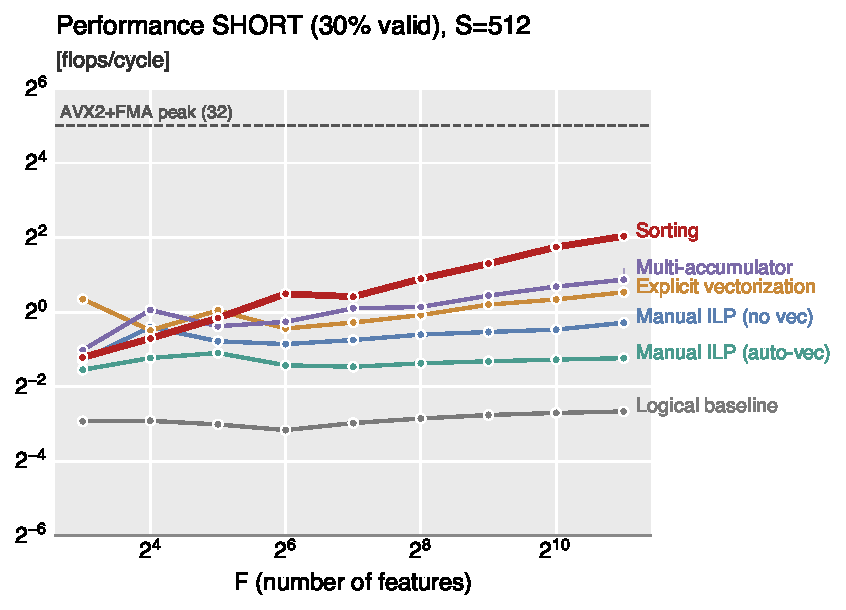
\includegraphics[width=0.48\linewidth]{figures/generated/perf_SHORT.pdf} 
  \\[1mm] % Explicit newline with controlled spacing
  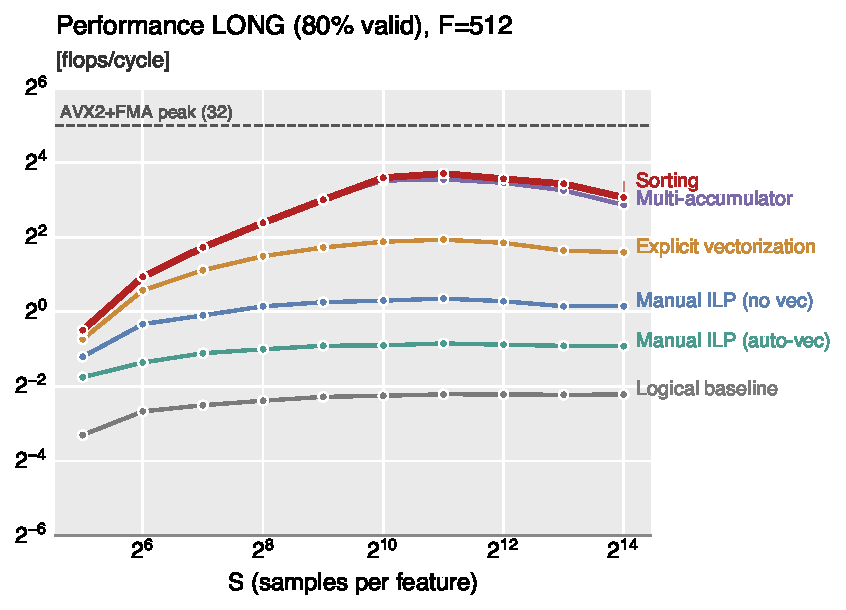
\includegraphics[width=0.48\linewidth]{figures/generated/perf_S_LONG.pdf}
  \hfill
  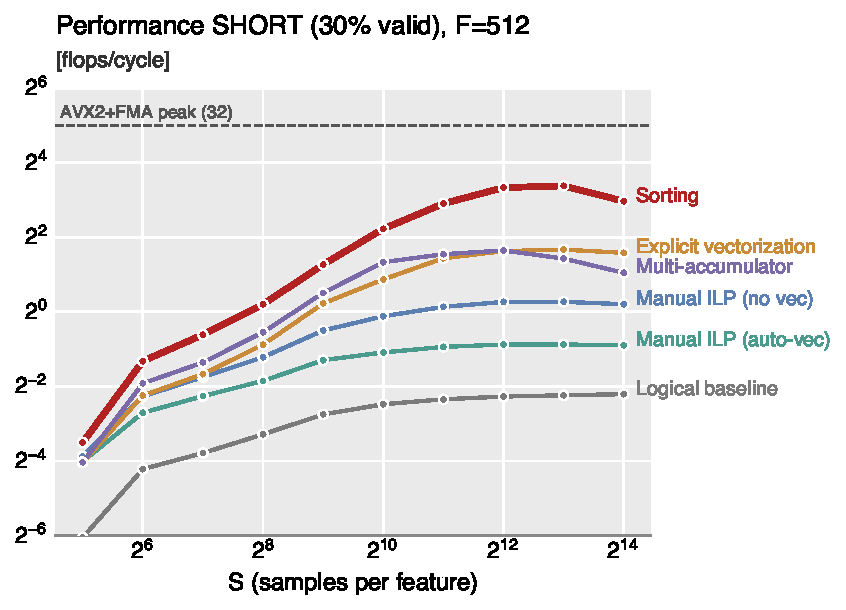
\includegraphics[width=0.48\linewidth]{figures/generated/perf_S_SHORT.pdf}
  
  \vspace{-3mm}
  \caption{Effective performance [flops/cycle] versus different input parameters. The two left figures are for \texttt{LONG} and the right figures are for \texttt{SHORT}. The upper half shows the different number of features $F$ at $S=512$, and the lower half shows the different number of samples per feature $S$ at $F=512$. Both axes are $\log_2$-scaled.}
  \label{fig:perf}
  
  \vspace{4.5mm}
  
  % --- FIGURE 2 (Rooflines) ---
  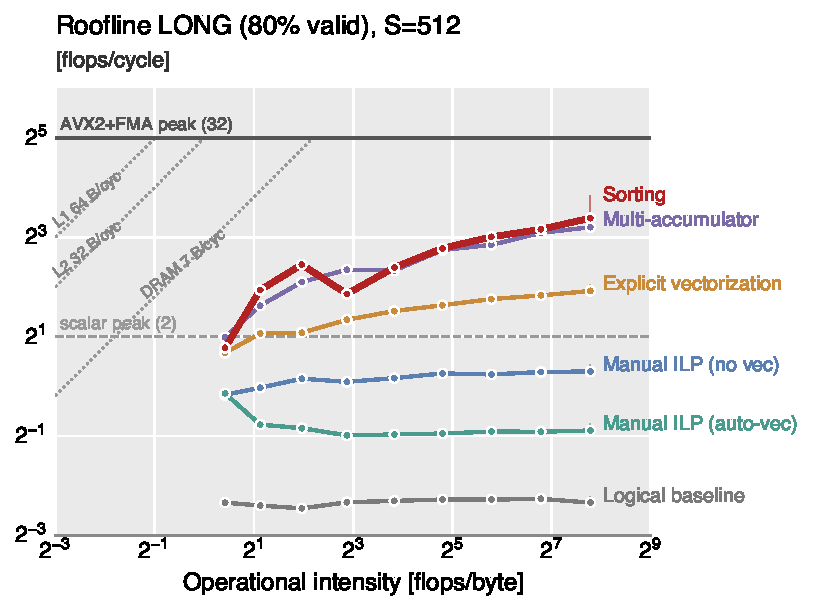
\includegraphics[width=0.48\linewidth]{figures/generated/roofline_LONG.pdf}
  \hfill
  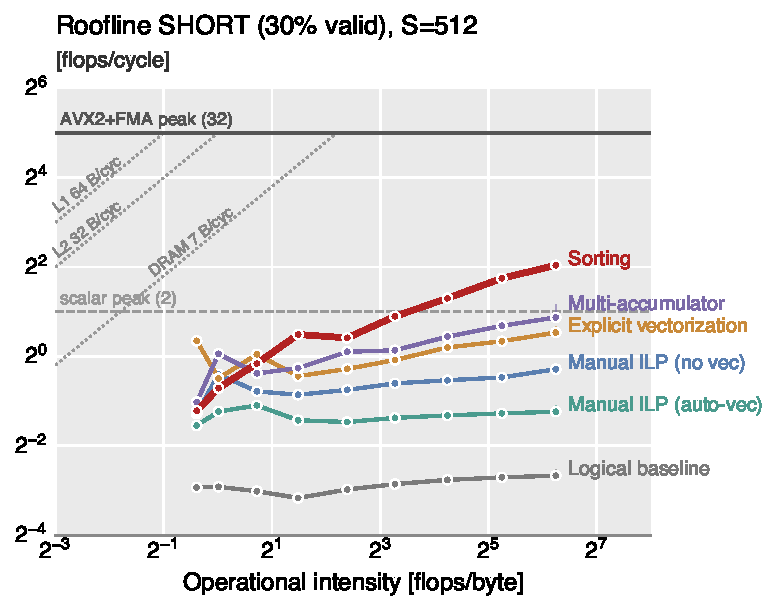
\includegraphics[width=0.48\linewidth]{figures/generated/roofline_SHORT.pdf} 
  \\[1mm] % Explicit newline with controlled spacing
  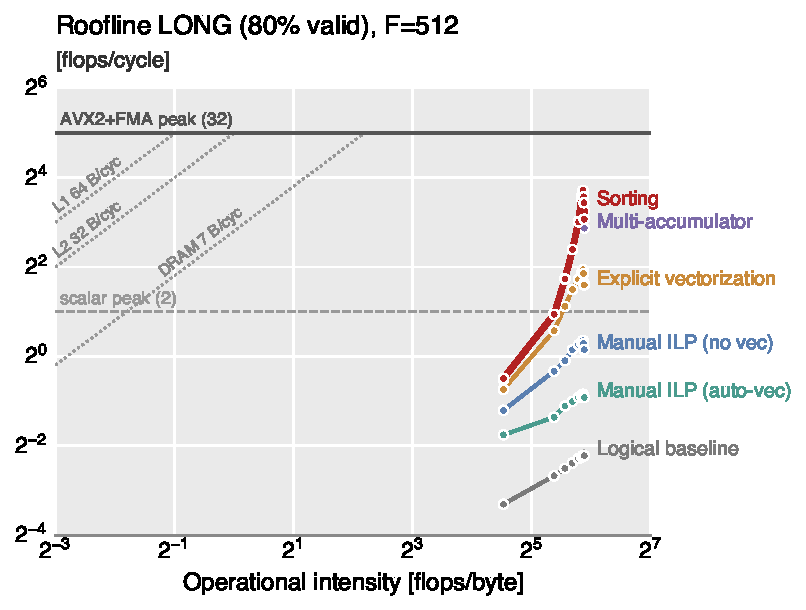
\includegraphics[width=0.48\linewidth]{figures/generated/roofline_S_LONG.pdf}
  \hfill
  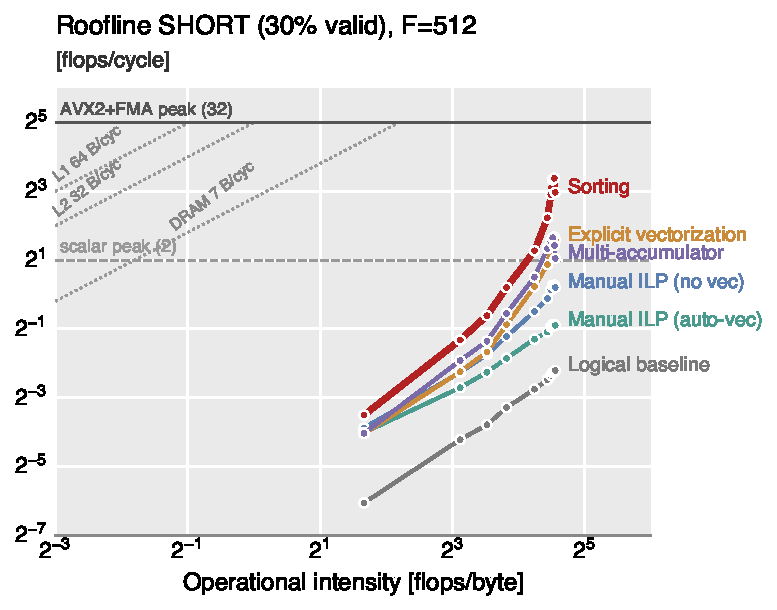
\includegraphics[width=0.48\linewidth]{figures/generated/roofline_S_SHORT.pdf}
  
  \vspace{-3mm}
  \caption{Rooflines for the \texttt{LONG} (left) and \texttt{SHORT} (right). Each dot is one $F\in\{8,16,\dots,2048\}$ at $S=512$ (up, F-sweep), or one $S\in\{32,64,\dots,16384\}$ at $F=512$ (down, S-sweep). Operational intensity is the analytical flop-to-compulsory-byte ratio of the cost model.}
  \label{fig:roofline}
  
\end{figure*}

% \begin{figure*}[h]
%   \centering
%   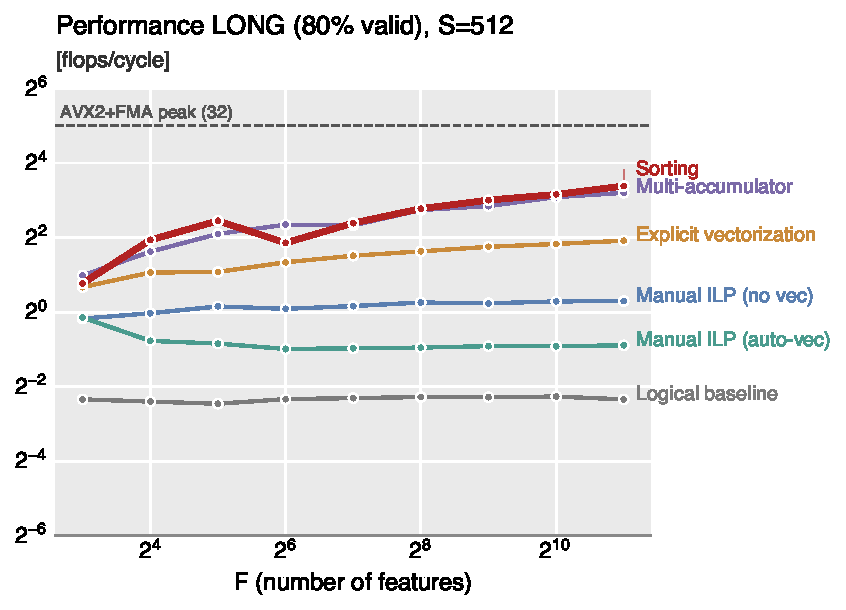
\includegraphics[width=0.48\linewidth]{figures/generated/perf_LONG.pdf}
%   \hfill
%   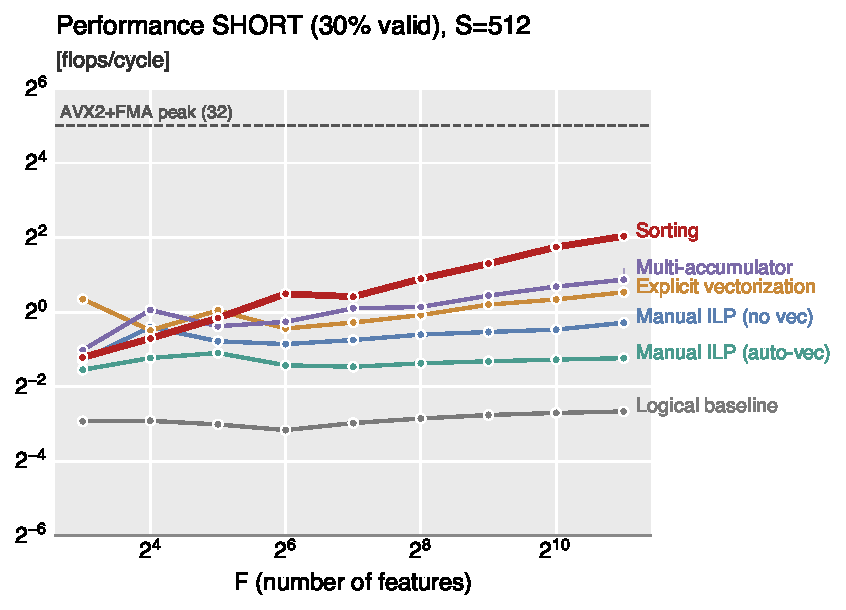
\includegraphics[width=0.48\linewidth]{figures/generated/perf_SHORT.pdf}
%   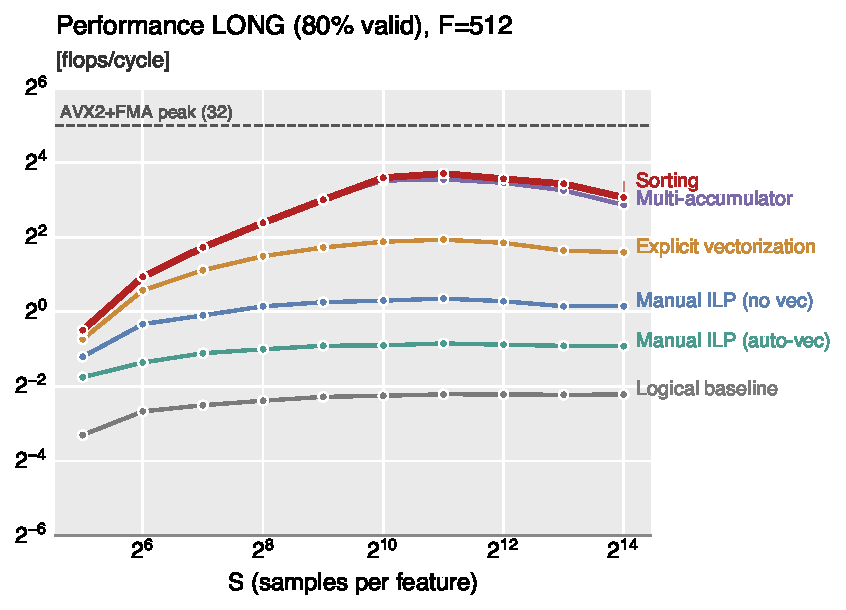
\includegraphics[width=0.48\linewidth]{figures/generated/perf_S_LONG.pdf}
%   \hfill
%   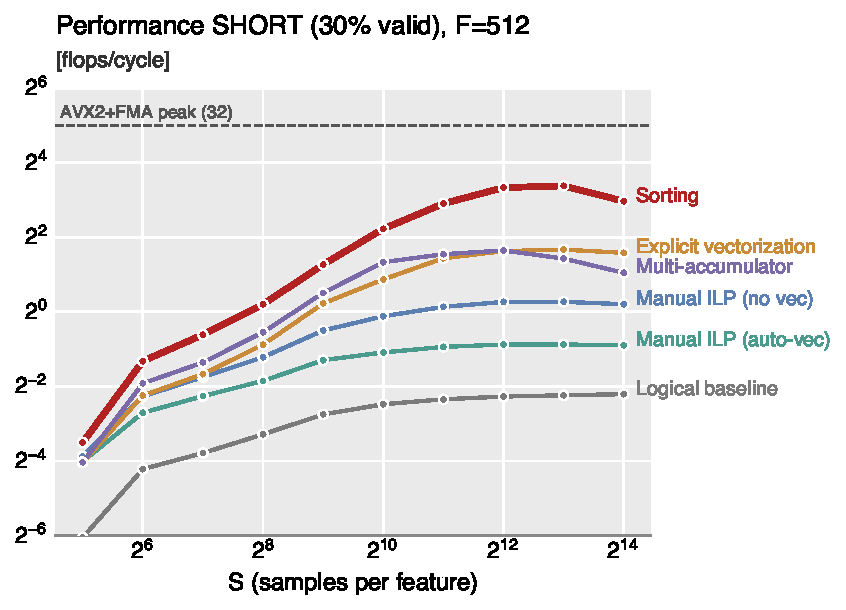
\includegraphics[width=0.48\linewidth]{figures/generated/perf_S_SHORT.pdf}
%   \caption{Effective performance [flops/cycle] versus different input parameters. The two left figures are for \texttt{LONG} and the right figures are for \texttt{SHORT}. The upper half shows the different number of features $F$ at $S=512$, and the lower half shows the different number of samples per feature $S$ at $F=512$. Both axes are $\log_2$-scaled.}
%   \label{fig:perf}
% \end{figure*}

% \begin{figure*}[t]
%   \centering
%   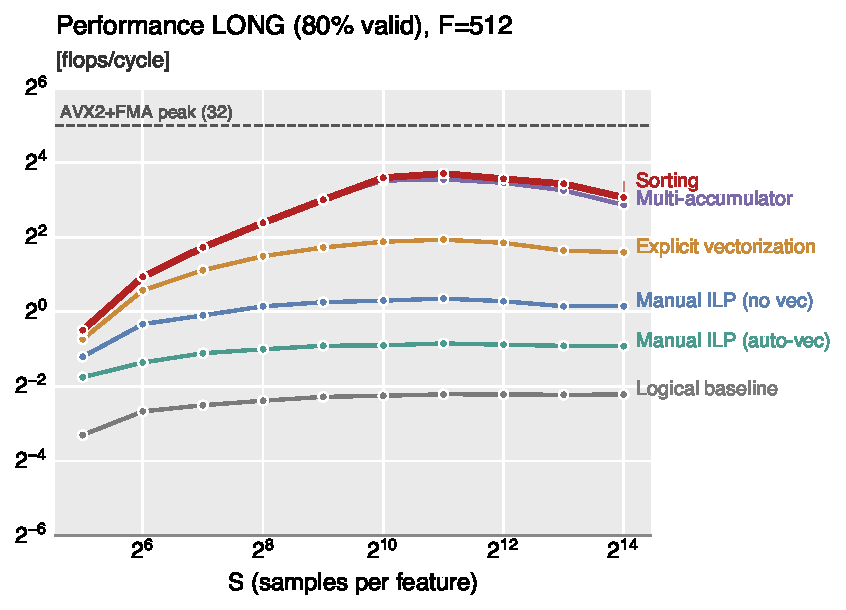
\includegraphics[width=0.48\linewidth]{figures/generated/perf_S_LONG.pdf}
%   \hfill
%   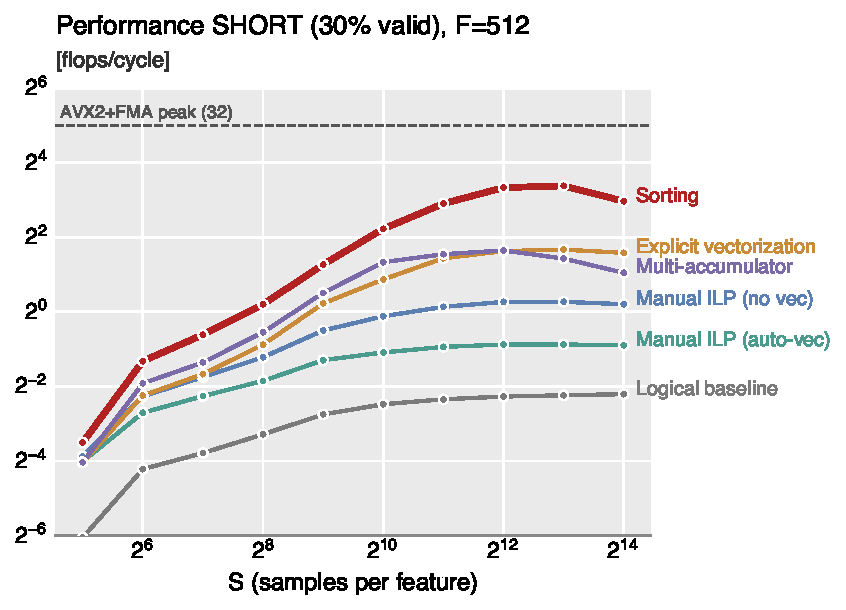
\includegraphics[width=0.48\linewidth]{figures/generated/perf_S_SHORT.pdf}
%   \caption{Effective performance [flops/cycle] versus the number of samples per feature $S$ at $F=512$ in the \texttt{LONG} (left) and \texttt{SHORT} (right). Both axes are $\log_2$.}
%   \label{fig:perf_S}
% \end{figure*}

% \begin{figure*}[h]
%   \centering
%   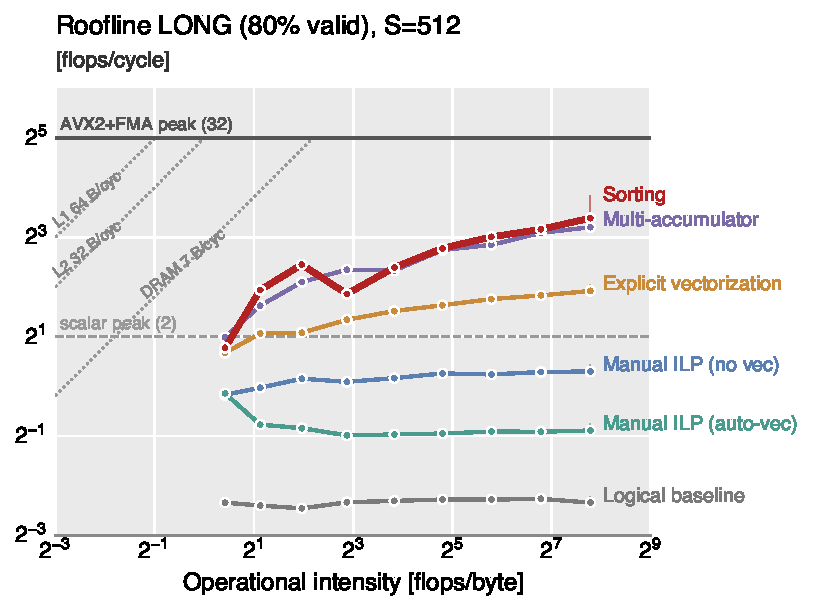
\includegraphics[width=0.48\linewidth]{figures/generated/roofline_LONG.pdf}
%   \hfill
%   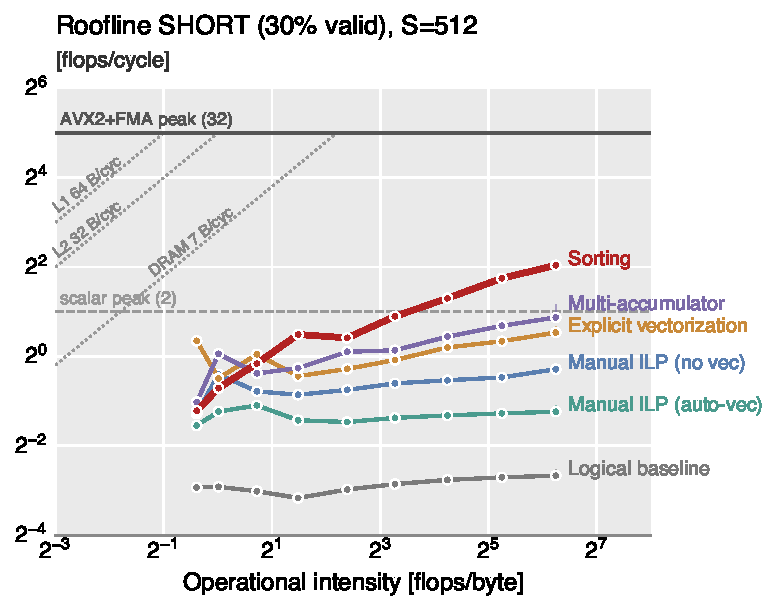
\includegraphics[width=0.48\linewidth]{figures/generated/roofline_SHORT.pdf}
%   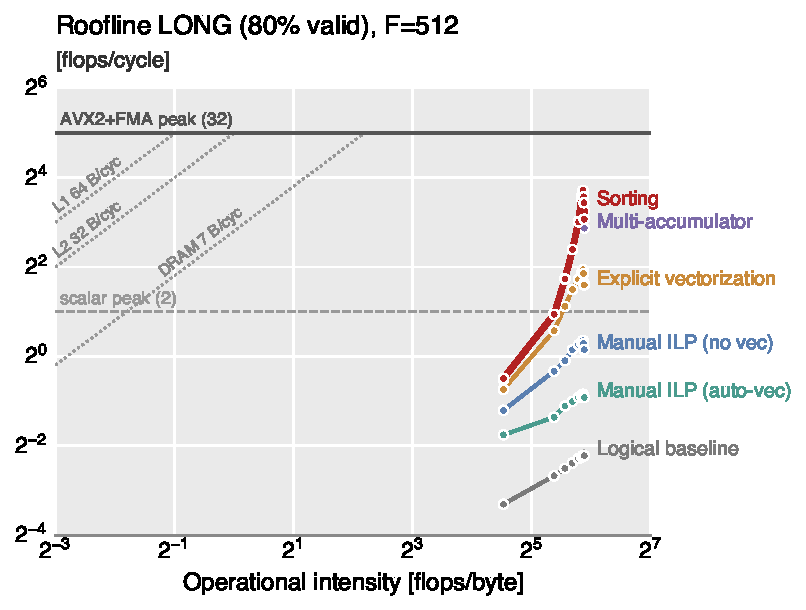
\includegraphics[width=0.48\linewidth]{figures/generated/roofline_S_LONG.pdf}
%   \hfill
%   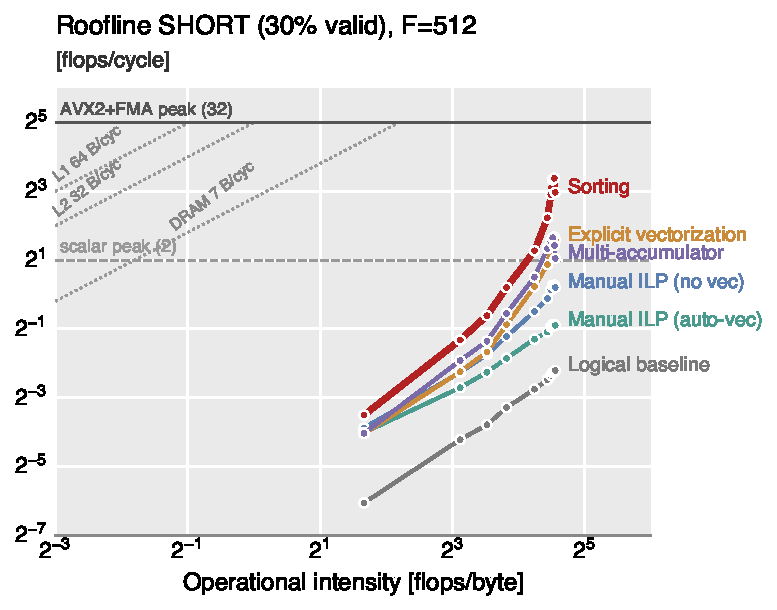
\includegraphics[width=0.48\linewidth]{figures/generated/roofline_S_SHORT.pdf}
  
%   \caption{Rooflines for the \texttt{LONG} (left) and \texttt{SHORT} (right). Each dot is one $F\in\{8,16,\dots,2048\}$ at $S=512$ (up, F-sweep), or one $S\in\{32,64,\dots,16384\}$ at $F=512$ (down, S-sweep). Operational intensity is the analytical flop-to-compulsory-byte ratio of the cost model.}
%   \label{fig:roofline}
% \end{figure*}

% \begin{figure*}[t]
%   \centering
%   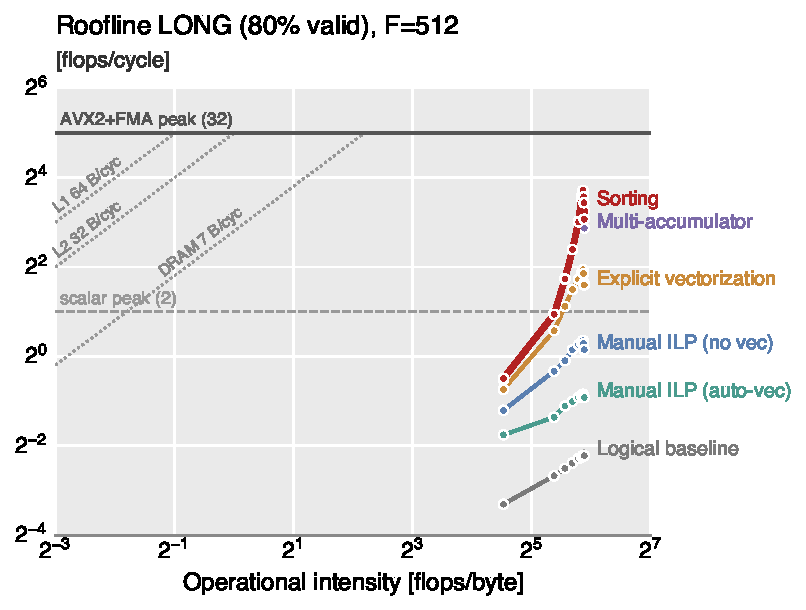
\includegraphics[width=0.48\linewidth]{figures/generated/roofline_S_LONG.pdf}
%   \hfill
%   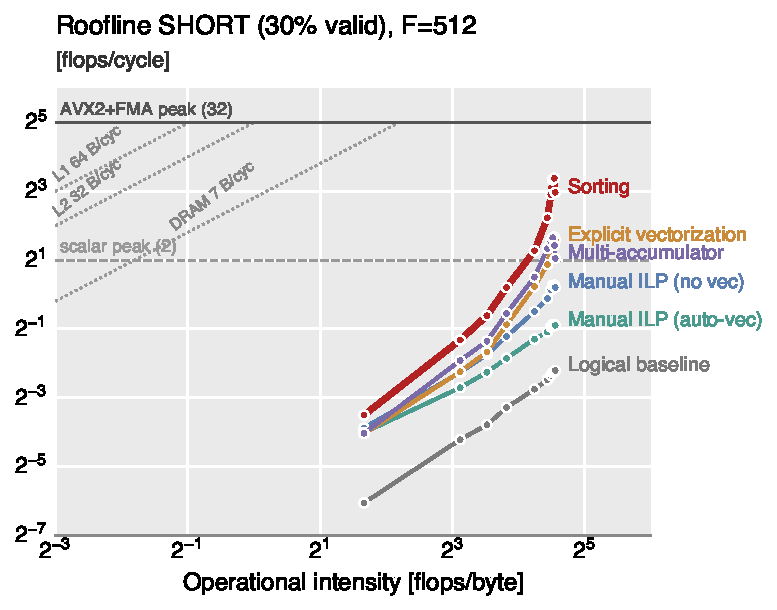
\includegraphics[width=0.48\linewidth]{figures/generated/roofline_S_SHORT.pdf}
%   \caption{Roofline for the \texttt{LONG} (left) and \texttt{SHORT} (right) when sweeping $S\in\{32,\dots,16384\}$ at $F=512$; each dot is one $S$, connected in order. Larger $S$ raises operational intensity and moves the best variant up toward AVX2+FMA peak.}
%   \label{fig:roofline_S}
% \end{figure*}

\begin{table*}[t]
  \centering
  \footnotesize
  \caption{PAPI hardware counters for each step at $F=2048$, $S=512$, medians over the timed batches. \texttt{Perf} is analytical flops per cycle, \texttt{IPC} is instructions per cycle, and \texttt{ins/flop} is the instruction per real flop count not the analytical. \texttt{L* mss} is the different cache level misses and  \texttt{\%stl} is the fraction of cycles the core was stalled.}
  \label{tab:papi}
  \begin{tabular}{l rrrrrr @{\hskip 2.2em} rrrrrr}
    \toprule
    & \multicolumn{6}{c}{\texttt{LONG} ($80\%$ valid)} & \multicolumn{6}{c}{\texttt{SHORT} ($30\%$ valid)}\\
    \cmidrule(lr){2-7}\cmidrule(lr){8-13}
    Step & perf & IPC & \shortstack{ins/\\flop} & \shortstack{L2\\miss} & \shortstack{L3\\miss} & \%stl & perf & IPC & \shortstack{ins/\\flop} & \shortstack{L2\\miss} & \shortstack{L3\\miss} & \%stl\\
    \midrule
    1 Logical baseline        & 0.20 & 2.71 & 13.8 & 131M & 0.67M & 16 & 0.16 & 2.47 & 15.7 & 31M & 0.17M & 17\\
    2 Manual ILP (no vec)     & 1.23 & 3.32 & 2.7  & 128M & 1.27M &  2 & 0.82 & 2.55 & 3.1  & 31M & 0.18M &  8\\
    3 Manual ILP (auto-vec)   & 0.54 & 1.65 & 3.1  & 130M & 1.36M & 32 & 0.42 & 1.66 & 3.9  & 28M & 0.20M & 22\\
    4 Explicit vectorization  & 3.78 & 1.93 & 0.51 & 111M & 1.37M & 31 & 1.45 & 1.41 & 0.98 & 29M & 0.17M & 11\\
    5 Multi-accumulator       & 9.19 & 2.28 & 0.25 &  27M & 0.25M & 27 & 1.83 & 2.12 & 1.16 & 16M & 0.18M & 24\\
    6 Sorting                 &10.43 & 2.25 & 0.22 &  21M & 0.39M & 29 & 4.11 & 1.86 & 0.45 & 4.3M& 0.14M & 23\\
    \bottomrule
  \end{tabular}
\end{table*}

\mypar{Per-step gains with the number of features}
Figure~\ref{fig:perf} (upper half) shows each optimization's performance and Table~\ref{tab:papi} gives the PAPI counters behind each line at $F=2048$ to attribute every change to a concrete cause. Unless stated otherwise we quote the dense \texttt{LONG} regime at $F=2048$ for consistency. The logical baseline sits far below every other line, at only $0.20$ flops/cycle. Compiled at \texttt{-O0}, it executes $13.8$ instructions for every useful flop, so even though it sustains an IPC of $2.7$, almost all of that work is loads and memory accesses rather than arithmetic. At this stage the bottleneck is the instruction count, not the hardware.

Manual ILP with four independent accumulators, still scalar, gives the largest relative jump of performance of $6.2\times$, to $1.23$ flops/cycle. Two effects combine here. \texttt{-O3} strips out the redundant instructions, dropping the instruction-per-flop ratio from $13.8$ to $2.7$, and the four accumulators break the loop-carried dependency in the Phase-2 reduction, lifting the IPC to $3.3$. The single accumulator in baseline forced each FMA to wait for the previous one. Now with four partial sums the core always has independent work to issue, achieving the desired instruction-level parallelism. This is the fastest purely scalar code we obtained.

The third line is counter-intuitive. Its source is identical to the previous step; the only change is that we stop passing \texttt{-fno-tree-vectorize}, letting the compiler auto-vectorize. Instead of improving, performance almost halves, to $0.54$ flops/cycle, and the IPC falls to $1.7$. The resource-stall fraction jumps from $1.6\%$ for the hand-tuned scalar loop to $32\%$ once the compiler vectorizes, so the core now spends roughly a third of its cycles stalled. The generated assembly explains it: GCC does vectorize the loop, but because the interval bounds are not known at compile time, it surrounds the vector loop with scalar code that handles the few elements at the start and end one at a time and adds shuffle instructions to line the data up. This kernel does not therefore auto-vectorize well, and the gains have to come from vectorizing by hand. Doing so with explicit AVX2/FMA achieves $3.78$ flops/cycle ($19\times$). Padding the invalid entries with zeros, turns the masked dot product into a dense, branch-free eight-wide one, and the instruction-per-flop ratio drops to $0.51$, about one instruction per two useful flops. The bottleneck now is that we fold everything into one vector accumulator, which reintroduces the loop-carried dependency we had removed, this time on the vector FMA, so the IPC is only $1.9$.

Multi-accumulator $4\times2$ register blocking breaks that loop-carried dependency and cuts the memory traffic at the same time. We obtain a performance of $9.19$ flops/cycle ($47\times$). Computing a $4\times2$ block of feature pairs at once gives eight independent FMA chains. Since an FMA on this core has a four-cycle latency and the two FMA units can each start one per cycle, roughly eight need to be in flight to keep both units busy, and eight is exactly what the block provides, so the IPC increases to $2.3$. Just as important, each loaded vector is now reused across all the pairs in the block instead of being re-read from memory for every single pair, and the cache counters show this directly: L2 misses drop by $4.2\times$ and L3 misses by $5.5\times$.

Finally, sorting the features by interval start adds another $13\%$ in \texttt{LONG}, to $10.43$ flops/cycle ($53\times$ overall). Here every pair already overlaps so there is nothing to skip, and the gain comes only from processing features in sorted order, which makes the accesses contiguous and predictable for the hardware prefetcher and removes a further $20\%$ of the L2 misses. Note that this is different for the \texttt{SHORT} as explained next.

\mypar{Why the \texttt{LONG} and \texttt{SHORT} differ}
The upper right panel of Figure~\ref{fig:perf} looks quite different. In \texttt{SHORT}, multi-accumulator reaches only $1.83$ flops/cycle, barely above explicit vectorization, yet sorting more than doubles it to $4.11$ ($26\times$ end-to-end). Comparing the flop counts from PAPI against the analytical useful-flop count gives a ratio of $4.8$ for multi-accumulator in \texttt{SHORT}, against only $1.19$ in \texttt{LONG}. In other words, the dense block always computes the full row length regardless of the real overlap, so on the short \texttt{SHORT} intervals it spends almost five hardware flops per useful flop, wasting FMA slots on padded zeros. The early-exit test that sorting enables skips the roughly $40\%$ of pairs that do not overlap at all and trims the padded tails, dropping the padding factor back to $1.08$ and accounting for essentially the entire $1.83\to4.11$ improvement. The cache counters confirm the same effect from the memory side, with sorting cutting \texttt{SHORT} L2 misses from $16$M to $4.3$M. In \texttt{LONG} the overlaps are dense and the padding overhead is not noticeable, only 3\%. Sorting is therefore the one optimization whose payoff is dictated by the shape of the input rather than by the hardware.

\mypar{Scaling with the dot-product length}
Figure~\ref{fig:perf} (lower half) fixes $F=512$ and grows $S$, the length of each dot product. The work done for one pair of features splits into two parts. The first is the dot product itself, whose length grows with $S$, so the longer the overlap, the more multiply-adds we perform. The second is a fixed amount of aggregation, i.e. summing the eight lanes of the vector accumulator into a single number, doing one division, and pushing the result into the top-$K$ heap of each of the two features. This tail costs the same handful of instructions regardless of $S$, because it does not depend on how long the dot product was. This split shapes the curve. When $S$ is small, the short dot product loop means the constant tail dominates the per-pair time and most cycles go there rather than to FMAs, keeping the initial performance low. As $S$ grows the dot product lengthens while the tail stays fixed, amortizing the cost over more useful work; this is why every curve climbs steeply at first. The climb does not continue forever, because a second effect eventually takes over. The best \texttt{LONG} variant peaks at $13.1$ flops/cycle ($41\%$ of peak) at $S=2048$, the largest size at which the whole normalized matrix ($F\cdot S\cdot4 = 4$\,MB) still fits inside the $6$\,MB L3 cache and is therefore served from cache. Beyond this ($8$\,MB at $S=4096$, $32$\,MB at $S=16384$), the matrix has to be streamed from main memory on every pass, dropping performance back to $8.4$ flops/cycle as DRAM bandwidth, rather than the tail, becomes the limit. \texttt{SHORT} peaks later, at $S=8192$, because its overlaps are shorter. At the same $S$, its dot product processes fewer valid samples and requires a larger $S$ to hide the same fixed tail. This means that once the algorithm is fast enough to be limited by computation, the bottleneck is on the constant work part 2 and not the dot product.

\mypar{Roofline analysis}
While the performance plots show how fast we are, the roofline in Figure~\ref{fig:roofline} shows whether we are limited by computation or by memory. We compute operational intensity (OI) as the analytical flop count divided by the algorithm's compulsory memory traffic, and the $y$-axis reuses the same cold-cache cycle counts as before. The ridge point, where the memory roof meets the compute roof, sits at $\approx4.6$ flops/byte. We measure the memory bandwidth of $7$\,B/cycle from a single-core STREAM-triad measurement of $19.8$\,GB/s at $2.8$\,GHz. Reading the $F$-sweep plots (upper half) from left to right, at small sizes start under the memory roof: at $F=8$ the OI is only $1.3$ in \texttt{LONG} and $0.76$ in \texttt{SHORT}, below the ridge, so there the algorithm is memory-bound and no amount of vector tuning would help. As $F$ grows the dots march to the right because each loaded row is reused across more pairs. The useful flops grow like $F^2$ while the compulsory memory access grows only like $F$, so OI climbs to $220$ in \texttt{LONG} and $76$ in \texttt{SHORT} and the whole working point moves into the compute-bound roof. At the sizes we care about, the DRAM bandwidth is not the limit anymore, making it legitimate to keep optimizing computation. The best \texttt{LONG} point lands at $10.4$ flops/cycle, $33\%$ of the AVX2+FMA roof. The $S$-sweep roofline in Figure~\ref{fig:roofline} (lower half) tells the same story from the other direction. Longer dot products raise OI and push the best variant up toward the roof, more steeply in \texttt{LONG} than in \texttt{SHORT}.

\mypar{Limitations}
Being limited by computation but still at only a third of peak means the bottleneck is now inside our algorithm implementation rather than in the memory system. We run a per-phase microbenchmark of the best variant and we saw that Phase 2 (pairwise correlation) takes $97.8\%$ of the cycles in \texttt{LONG} and $94.8\%$ in \texttt{SHORT}, while the normalization (Phase 1) and the heap read-out (Phase 3) together stay under $5\%$ and the sort itself under half a percent. Almost all of that Phase-2 time is the inner pair loop, so this is the only place where remaining headroom can be found. Within that loop, we saw that the division is the most expensive piece. It is a scalar single-precision divide done once for every feature pair inside the Phase-2 loop nest (the $\textnormal{acc}/(N-1)$ that turns each finished dot product into a correlation), and on this core a division is a long-latency operation that the hardware does not pipeline the way it overlaps the multiply-adds, so we cannot hide the latency. Crucially, we only do this division once per feature pair regardless of the overlap length. We also checked that the zero padding we added is not the bottleneck. We saw that after sorting the algorithm does only about $8\%$ more floating-point work than strictly necessary. In short, the two FMA units are already saturated by the dot product, so the ceiling is set by this serial, scalar tail that we run once per pair and cannot widen to vectors or hide behind the multiply-adds.

\section{Conclusions}
Starting from a logical baseline that already exploited symmetry and a numerically stable variance formulation, we took the Interval-Masked Top-$K$ Pearson correlation algorithm through different optimization and reached $10.4$ flops/cycle, $33\%$ of the AVX2+FMA peak, for a $53\times$ speedup on dense intervals and $26\times$ on sparse ones. Two findings stand out. First, the masked inner loop did not auto-vectorize usefully, that is, letting the compiler vectorize it was actually slower than clean scalar code, and the real gains came only once we vectorized by hand on top of a zero-padding scheme that made the masked dot product dense and branch-free. Second, the value of an optimization depended heavily on the input data, with interval sorting almost irrelevant on dense data but the single most important step on sparse data, where its early exit removed the wasted work the padding introduced. The roofline showed that at the problem sizes of interest the kernel is limited by computation rather than by memory bandwidth, and a per-phase microbenchmark localized the remaining gap to peak inside the Phase-2 pair loop, which alone accounts for over $94\%$ of the runtime: not the vectorized dot product, which already keeps both FMA units busy. The main bottleneck still is on the fixed scalar work done once per feature pair, dominated by the long-latency division that normalizes each finished dot product.

% \section{Check list}

% Here we summarize main points and provide some further tips.

% \mypar{Important}

% \begin{itemize}
% \item Make sure to have a cost analysis or (in rare cases) argue why not and what you do instead.

% \item Be analytical in explaining your results and limitations as this is a crucial factor for the grade.

% \item {\color{red} Make sure to report the fastest non-vectorized code you obtained, compiled with flags disabling compiler vectorization. Also report the best compiler-vectorized code.}

% \item Plots should be readable. A plot can look fine when created but once put in one column you may have 4 point font, which is way to small. See also the small benchmarking guide I presented.

% \item If you show a roofline plot, explain exactly how you got the data for it and the assumptions (e.g., on cache state). Revisit the roofline lecture on do's and dont's.

% \item Don't talk about unrolling as performance optimization (see lectures where this is discussed several times) but be precise.

% \item Some infrastructure work for testing and timing is needed but does not count towards the grade. Every project member has to contribute optimizations or relevant analyses.

% \item No tricks to save space in latex (squeezing font or the like).
% \end{itemize}

% \mypar{Some tips}
% \begin{itemize}
% \item For short papers like this, to save space, I use paragraph titles instead of subsections, as shown in the introduction.

% \item It is generally a good idea to break sections into such smaller
% units for readability and since it helps you to (visually) structure the story.

% \item The above section titles should be adapted to more precisely
% reflect what you do, and structure can be changed if it makes sense.

% \item Each section should be started with a very
% short summary of what the reader can expect in this section.

% \item Do not use subsubsections.

% \item Make sure you define every acronym you use, no matter how
% convinced you are the reader knows it.

% \item Always spell-check before you submit.

% \item Also strive for reasonably high visual quality of the report.
% In this class, the quality also contributes to the grade.

% \item Books helping you to write better: \cite{Higham:98} and \cite{Strunk:00}.
% \end{itemize}

% \mypar{Graphics} Fig.~\ref{fftperf} is an example plot that I used in a lecture. Note that the fontsize in the plot should not be any smaller. On the other hand it is also a good rule that the font size in the plot is not larger than the one in the caption (otherwise it looks ugly).

% \begin{figure}\centering
%   \includegraphics[scale=0.33]{dft-performance.pdf}
%   \caption{Performance of four single-precision implementations of the
%   discrete Fourier transform. The operations count is roughly the
%   same. {\em The labels in this plot are about the smallest you should go.}\label{fftperf}}
% \end{figure}

% \bigskip
% {\bf Up to here you have 7 pages and you should use them well.}

% \bigskip
% After the 7 pages there should be no appendix (will be ignored by us) but please include the mandatory sections explained after the bibliography.

% References should be produced using the bibtex program from suitable
% BiBTeX files (here: bibl_conf). The IEEEbib.bst bibliography
% style file from IEEE produces unsorted bibliography list.
% -------------------------------------------------------------------------

\bibliographystyle{IEEEbib}
\bibliography{bibl_conf}

\newpage
\clearpage
\section{Contributions of Team Members (Mandatory)}
% {\color{gray}
%     In this mandatory section (which is not included in the 7 pages limit) each team member should very briefly (telegram style is welcome) explain what she/he did for the project in terms of optimizations {\bf (do not mention  infrastructure work on testing and timing)}. I imagine this section to be maximally one column, rather less.

%     Include only
%     \begin{itemize}
%     	\item What relates to optimizing your chosen algorithm / application. This means writing actual code for optimization or for analysis.
%     	\item What you did before the submission of the presentation.
%     \end{itemize}
%     Do not include
%     \begin{itemize}
%     	\item Work on infrastructure and testing.
%     	\item Work done after the presentation took place.
%     \end{itemize}
% }

\mypar{Luhao} Implemented the explicit AVX2/FMA vectorization of the Phase-2 dot product (step~4) and the Phase-3 min-heap. Came up with the "logical" optimizations in the logical baseline (step~1).

\mypar{Andres} Wrote and implemented the decomposed incremental stages (the manual-ILP variants with and without auto-vectorization, steps~2 and~3, and the interval-sorting step, step~6). Imporved the vectorization solution to exploit full hardware. Study the performance of each algorithm to understand the bottlenecks.

\mypar{Oliver} Performance and roofline analysis across all variants plus the plotting, analyzing the isolated effect of each optimization stage. Helped implement 4x2 register blocking; came up with the interval-sorting idea.


\section{Code (Mandatory)}\label{sec:code}
This section does not count towards the 7 pages limit.

Please copy-paste the most performance-critical part of your fastest scalar code here. Should be at most one page. If you have more than one such part, choose one. Could be done in single column if need be. For best display consider adding a page break in latex before.

Paste in here, do not change font size:
% // Phase 1
% for (uint32_t i = 0; i < F; i++) {
%   uint32_t start = starts[i];
%   uint32_t end = ends[i];
%   uint32_t n = end - start;

%   float sum0 = 0.0f, sum1 = 0.0f, 
%     sum2 = 0.0f, sum3 = 0.0f;
%   float sq0 = 0.0f, sq1 = 0.0f, 
%     sq2 = 0.0f, sq3 = 0.0f;

%   uint32_t j = start;
%   uint32_t end4 = start + (n & ~3u);
%   for (; j < end4; j += 4) {
%     float x0 = X[i * S + j];
%     float x1 = X[i * S + j + 1];
%     float x2 = X[i * S + j + 2];
%     float x3 = X[i * S + j + 3];
%     sum0 += x0;
%     sum1 += x1;
%     sum2 += x2;
%     sum3 += x3;
%     sq0 += x0 * x0;
%     sq1 += x1 * x1;
%     sq2 += x2 * x2;
%     sq3 += x3 * x3;
%   }
%   for (; j < end; j++) {
%     sum0 += X[i * S + j];
%     sq0 += X[i * S + j] * X[i * S + j];
%   }

%   float sum = sum0 + sum1 + sum2 + sum3;
%   float sum_sq = sq0 + sq1 + sq2 + sq3;

%   float mean = sum / n;
%   float var =
%     (((n * mean) * mean) - ((2.0f * sum) * mean) + sum_sq) 
%     / (n - 1);
%   float std = sqrt(var + STD_EPS);

%   for (uint32_t j = start; j < end; j++) {
%     normalized_X[i * S + j] = (X[i * S + j] - mean) / std;
%   }
% }
{\fontsize{8}{10}\selectfont
\begin{Verbatim}
// Phase 2
for (uint32_t i = 0; i < F; i++) {
  for (uint32_t j = i + 1; j < F; j++) {
    uint32_t start = std::max(starts[i], starts[j]);
    uint32_t end = std::min(ends[i], ends[j]);

    uint32_t n = end - start;
    if (n < 2) {
      continue;
    }

    float acc0 = 0.0f, acc1 = 0.0f, 
      acc2 = 0.0f, acc3 = 0.0f;

    uint32_t k = start;
    uint32_t end4 = start + (n & ~3u);
    for (; k < end4; k += 4) {
      acc0 += normalized_X[i * S + k] * 
        normalized_X[j * S + k];
      acc1 += normalized_X[i * S + k + 1] * 
        normalized_X[j * S + k + 1];
      acc2 += normalized_X[i * S + k + 2] * 
        normalized_X[j * S + k + 2];
      acc3 += normalized_X[i * S + k + 3] * 
        normalized_X[j * S + k + 3];
    }
    for (; k < end; k++) {
      acc0 += normalized_X[i * S + k] * 
        normalized_X[j * S + k];
    }

    float corr = (acc0 + acc1 + acc2 + acc3) / (n - 1);
    float v = std::fabs(corr);

    heap_insert(&topK_heaps[i * K], v, j);
    heap_insert(&topK_heaps[j * K], v, i);
  }
}
\end{Verbatim}
}

After that, please paste the most performance-critical part of your fastest SIMD code here. Again, this should be at most one page. If you have more than one such part, choose one. Could be done in single column if need be. For best display consider adding a page break in latex before.

Paste in here, do not change font size:
% // Phase 1
% for (uint32_t si = 0; si < F; ++si) {
%   uint32_t orig_i = perm[si];
%   uint32_t start = starts[orig_i];
%   uint32_t end = ends[orig_i];
%   uint32_t aligned32_start = start & ~31u;
%   uint32_t aligned32_end = (end + 31u) & ~31u;
%   uint32_t aligned8_start = start & ~7u;
%   uint32_t aligned8_end = (end + 7u) & ~7u;
%   uint32_t interval_size = end - start;

%   // Math: variance_sum = sum((x - mean)^2) = 
%   // sum(x^2) - 2*mean*sum(x) + n*mean^2
%   float sum = 0.0f;
%   float sum_sq = 0.0f;
%   if (S >= 32) {
%     // Manual vectorization: 0.0 padding elements won't contribute to the
%     // sum Multiple accumulators: remove dependency chain
%     __m256 v_sum[4] = {_mm256_setzero_ps(), _mm256_setzero_ps(),
%                        _mm256_setzero_ps(), _mm256_setzero_ps()};
%     __m256 v_sum_sq[4] = {_mm256_setzero_ps(), _mm256_setzero_ps(),
%                           _mm256_setzero_ps(), _mm256_setzero_ps()};
%     const float *base_ptr = &X[orig_i * S + aligned32_start];
%     for (uint32_t j = aligned32_start; j < aligned32_end;
%       j += 32, base_ptr += 32) {
%       __m256 v_x[4] = {
%         _mm256_load_ps(base_ptr), _mm256_load_ps(base_ptr + 8),
%         _mm256_load_ps(base_ptr + 16), _mm256_load_ps(base_ptr + 24)
%       };
%       // v_sum += v_x
%       v_sum[0] = _mm256_add_ps(v_sum[0], v_x[0]);
%       v_sum[1] = _mm256_add_ps(v_sum[1], v_x[1]);
%       v_sum[2] = _mm256_add_ps(v_sum[2], v_x[2]);
%       v_sum[3] = _mm256_add_ps(v_sum[3], v_x[3]);
%       // v_sum_sq += v_x * v_x
%       v_sum_sq[0] = _mm256_fmadd_ps(v_x[0], v_x[0], v_sum_sq[0]);
%       v_sum_sq[1] = _mm256_fmadd_ps(v_x[1], v_x[1], v_sum_sq[1]);
%       v_sum_sq[2] = _mm256_fmadd_ps(v_x[2], v_x[2], v_sum_sq[2]);
%       v_sum_sq[3] = _mm256_fmadd_ps(v_x[3], v_x[3], v_sum_sq[3]);
%     }
%     v_sum[0] = _mm256_add_ps(v_sum[0], v_sum[1]);
%     v_sum[2] = _mm256_add_ps(v_sum[2], v_sum[3]);
%     v_sum_sq[0] = _mm256_add_ps(v_sum_sq[0], v_sum_sq[1]);
%     v_sum_sq[2] = _mm256_add_ps(v_sum_sq[2], v_sum_sq[3]);
%     v_sum[0] = _mm256_add_ps(v_sum[0], v_sum[2]);
%     v_sum_sq[0] = _mm256_add_ps(v_sum_sq[0], v_sum_sq[2]);
%     sum = hsum256_simple(v_sum[0]);
%     sum_sq = hsum256_simple(v_sum_sq[0]);
%   } else {
%     // Fallback to scalar code for small S
%     // (Skipped)
%   }

%   float variance_sum = ((interval_size * mean) * mean) +
%     ((-2.0f * sum) * mean + sum_sq); // FMA style
%   float std_sample =
%     std::sqrt(variance_sum / (interval_size - 1) + STD_EPS);
%   float inv_std_sample = 1.0f / std_sample;

%   // Precompute: normalized_X = (X - mean) / std_sample 
%   // for correlation computation
%   if (S >= 32) {
%     __m256 v_mean = _mm256_set1_ps(mean);
%     __m256 v_inv_std_sample = _mm256_set1_ps(inv_std_sample);
%     const float *base_ptr = &X[orig_i * S + aligned8_start];
%     float *normalized_ptr = &normalized_X[si * S + aligned8_start];
%     for (uint32_t j = aligned8_start; j < aligned8_end;
%       j += 8, base_ptr += 8, normalized_ptr += 8) {
%       __m256 v_x = _mm256_load_ps(base_ptr);
%       // v_normalized = (v_x - v_mean) * v_inv_std_sample
%       __m256 v_normalized =
%         _mm256_mul_ps(_mm256_sub_ps(v_x, v_mean), v_inv_std_sample);
%       _mm256_store_ps(normalized_ptr, v_normalized);
%     }
%   } else {
%     // Fallback to scalar code for small S
%     // (Skipped)
%   }
% }
{\fontsize{8}{10}\selectfont
\begin{Verbatim}
// Phase 2
// Pairwise correlation + top-K heap insertion (fused)
// Operates entirely on sorted rows

for (uint32_t i = 0; i < F; i += 4) {
  // Block processing: 
  // check 4 features at a time to have better locality

  // Original feature indices of the i-block
  // hoisted out of every inner heap_insert.
  uint32_t pi0 = perm[i];
  uint32_t pi1 = perm[i + 1];
  uint32_t pi2 = perm[i + 2];
  uint32_t pi3 = perm[i + 3];

  // Edge case (the diagonal staircase)
  // i   <-> i+1, i+2, i+3
  // i+1 <->      i+2, i+3
  // i+2 <->           i+3
  uint32_t l01 = std::max(sorted_starts[i], 
    sorted_starts[i + 1]);
  // Same for l02, l03, l12, l13, l23 (Skipped)
  uint32_t r01 = std::min(sorted_ends[i], 
    sorted_ends[i + 1]);
  // Same for r02, r03, r12, r13, r23 (Skipped)
  uint32_t n01 = r01 - l01;
  // Same for n02, n03, n12, n13, n23 (Skipped)

  uint32_t min_l = std::min(
    {l01, l02, l03, l12, l13, l23});
  uint32_t max_r = std::max(
    {r01, r02, r03, r12, r13, r23});

  __m256 acc01 = _mm256_setzero_ps();
  // Same for acc02, acc03, acc12, acc13, acc23 (Skipped)

  // min_l and max_r are multiples of 8
  const float *base_ptr = &normalized_X[i * S + min_l];
  for (uint32_t t = min_l; 
  t < max_r; t += 8, base_ptr += 8) {
    __m256 v_i0 = _mm256_load_ps(base_ptr);
    __m256 v_i1 = _mm256_load_ps(base_ptr + S);
    __m256 v_i2 = _mm256_load_ps(base_ptr + 2 * S);
    __m256 v_i3 = _mm256_load_ps(base_ptr + 3 * S);
    acc01 = _mm256_fmadd_ps(v_i0, v_i1, acc01);
    // Same for acc02, acc03, ..., acc23 (Skipped)
  }

  if (n01 > 0) {
    float tmp = std::fabs(
      hsum256_simple(acc01) / (n01 - 1));
    heap_insert(&topK_heaps[i * K], tmp, pi1);
    heap_insert(&topK_heaps[(i + 1) * K], tmp, pi0);
  }
  // Same for n02, n03, n12, n13, n23
  // (Skipped)


  // Hoist i-block end to drive the j-loop early-exit
  uint32_t i_block_max_end =
    std::max({sorted_ends[i], sorted_ends[i + 1], 
              sorted_ends[i + 2], sorted_ends[i + 3]});
  for (uint32_t j = i + 4; j + 1 < F; j += 2) {
    if (sorted_starts[j] >= i_block_max_end)
      break;
          
    uint32_t pja = perm[j];
    uint32_t pjb = perm[j + 1];
    // i, i+1, i+2, i+3 <-> (j, j+1)
    // 8 accumulators (4 i-features × 2 j-features) to 
    // keep 8 independent FMA dependency chains in 
    // flight saturates the 2-per-cycle FMA throughput  
    // on Skylake/Kaby Lake despite 4-cycle latency.
    uint32_t l0a = std::max(sorted_starts[i], 
      sorted_starts[j]);
    // Same for l1a, l2a, l3a, l0b, l1b, l2b, l3b 
    // (Skipped)
    uint32_t r0a = std::min(sorted_ends[i], 
      sorted_ends[j]);
    // Same for r1a, r2a, r3a, r0b, r1b, r2b, r3b 
    // (Skipped)
    uint32_t n0a = r0a - l0a, n1a = r1a - l1a, 
      n2a = r2a - l2a, n3a = r3a - l3a;
    uint32_t n0b = r0b - l0b, n1b = r1b - l1b, 
      n2b = r2b - l2b, n3b = r3b - l3b;

    uint32_t min_l = std::min(
      {l0a, l1a, l2a, l3a, l0b, l1b, l2b, l3b});
    uint32_t max_r = std::max(
      {r0a, r1a, r2a, r3a, r0b, r1b, r2b, r3b});

    __m256 acc0a = _mm256_setzero_ps();
    // Same for acc0a, ... (Skipped)
    
    // min_l and max_r are multiples of 8
    const float *base_ptr_i = 
      &normalized_X[i * S + min_l];
    const float *base_ptr_ja = 
      &normalized_X[j * S + min_l];
    const float *base_ptr_jb = 
      &normalized_X[(j + 1) * S + min_l];
    for (uint32_t t = min_l; t < max_r;
      t += 8, base_ptr_i += 8, 
      base_ptr_ja += 8, base_ptr_jb += 8) {
      __m256 v_i0 = _mm256_load_ps(base_ptr_i);
      __m256 v_i1 = _mm256_load_ps(base_ptr_i + S);
      __m256 v_i2 = _mm256_load_ps(base_ptr_i + 2 * S);
      __m256 v_i3 = _mm256_load_ps(base_ptr_i + 3 * S);
      __m256 v_ja = _mm256_load_ps(base_ptr_ja);
      __m256 v_jb = _mm256_load_ps(base_ptr_jb);
      acc0a = _mm256_fmadd_ps(v_i0, v_ja, acc0a);
      // Same for acc0b, acc1a, ..., acc3b (Skipped)
    }

    float s0a = hsum256_simple(acc0a), 
      s0b = hsum256_simple(acc0b);
    float s1a = hsum256_simple(acc1a), 
      s1b = hsum256_simple(acc1b);
    float s2a = hsum256_simple(acc2a), 
      s2b = hsum256_simple(acc2b);
    float s3a = hsum256_simple(acc3a), 
      s3b = hsum256_simple(acc3b);

    if (n0a > 0) {
      float v = std::fabs(s0a / (n0a - 1));
      heap_insert(&topK_heaps[i * K], v, pja);
      heap_insert(&topK_heaps[j * K], v, pi0);
    }
    // Same for n1a, n2a, n3a, n0b, n1b, n2b, n3b
    // (Skipped)

  }

  // Tail: handle the odd j=F-1 when the j-loop 
  // processed pairs evenly. The extra sorted_starts[F-1]
  // guard makes this a no-op when the j-loop early-exited 
  // (monotone sorted_starts means sorted_starts[F-1] >= 
  // i_block_max_end iff some j' <= F-1 already triggered
  // the early-exit).
  // (Edge Case: Skipped)
}
\end{Verbatim}
}

\end{document}
